%!TeX root=MemoriaTFG.tex
\chapter{Experimentacion}
En este capítulo se documentan las pruebas realizadas al aplicativo propuesto con el objetivo de analizar 
los resultados obtenidos del análisis y la simulación.

Esta experimentación parte de unas condiciones generales. Contamos con un total de 25 rutas reales 
realizadas en el territorio delimitado del Castell de Bellver (Illes Balears, España). Debido a que el 
número de muestras no es suficiente para representar un comportamiento se ha realizado un análisis y 
almacenando los resultados 7 veces por cada ruta real, de esta forma alimentamos el modelo con una 
cantidad de información suficiente para apreciar resultados. Estas condiciones de entrada parten de la
necesidad de alimentar el modelo con una información que pueda llegar a ser representativa.

En la figura \ref{figure:RealHeatMap} se muestra el mapa de calor resultado del proceso de análisis:
\begin{figure}[!htb]
\begin{center}
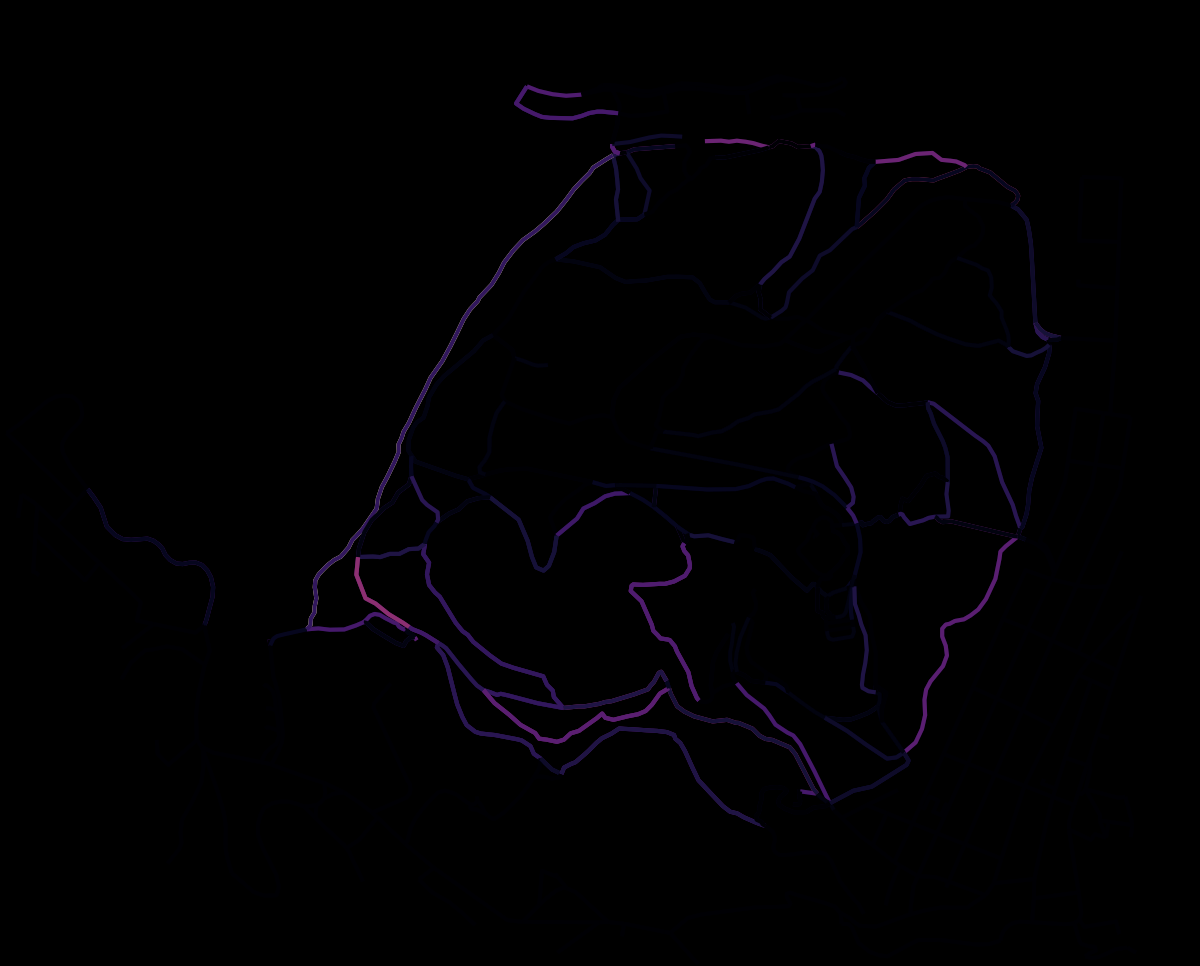
\includegraphics[width=0.7\textwidth]{./Imagenes/HeatMap.png}
\caption{Mapa de calor del conjunto de rutas reales.}
\label{figure:RealHeatMap}
\end{center}
\end{figure}
\newpage
Este mapa representa la frecuencia de paso del individuo por cada uno de los caminos establecidos en 
el territorio. Colores oscuros representarían frecuencias bajas y el color cobra una tonalidad rojiza a 
medida que la frecuencia sería mayor.

Se observa que el individuo ha realizado uso mayor del perímetro del bosque del territorio. Esto 
concuerda con la visualización de las rutas individuales. Con un conjunto mayor de datos, el mapa de 
calor llegaría a mostrar colores rojizos.

Las pruebas que realizaremos se basan en dos vertientes. Por una parte se realiza un análisis de una 
generación de rutas donde no se han importado datos reales. Por otro parte se realiza un análisis de 
rutas simuladas con datos reales introducidos en el modelo.


\section{Experimentación sin importación de datos reales}
En este apartado realiza la muestra de resultados de la generación de 10 rutas creadas 
mediante la simulación sin datos de análisis almacenados. Al no tener datos almacenados dentro del 
sistema la simulación corresponderá a una elección aleatoria del los diferentes caminos ya que, por 
defecto, todos los caminos tienen la misma probabilidad de tránsito a falta de introducir datos en el 
modelo. Por otra parte la distancia punto a punto será una constante definida en 20 metros, por lo 
que no aparecerá variabilidad en la muestra. Esta constante está parametrizada y puede ser 
modificable por el usuario.

Se han realizado una simulación de 10 rutas. El resultado son 10 ficheros \ac{GPX} que están situados en la carpeta X adjuntada con este documento.

\ref{figure:SimulatedTrack1}.
\begin{figure}[!htb]
\centering
\begin{minipage}{0.70\textwidth}
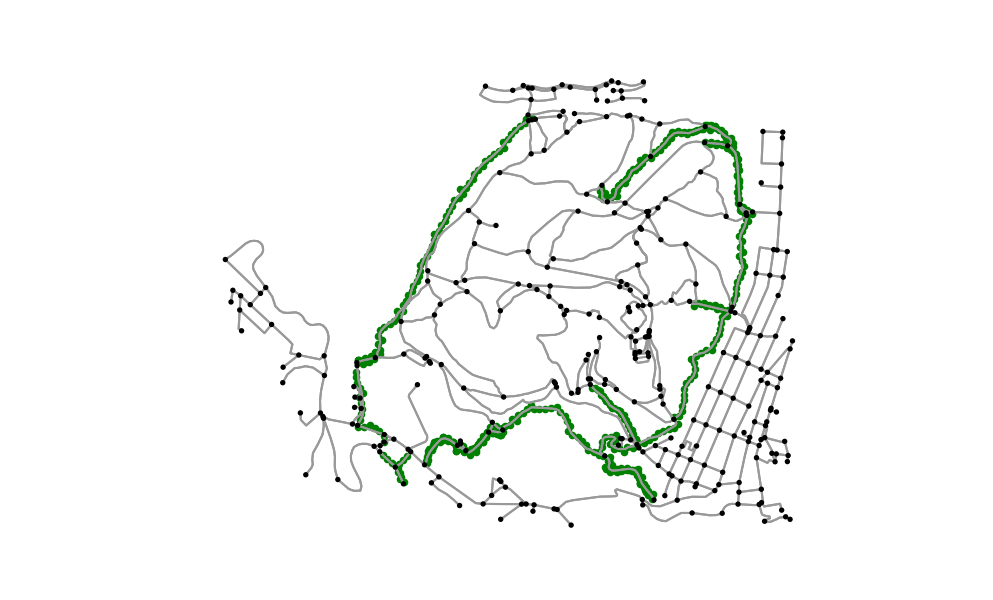
\includegraphics[width=0.9\textwidth]{./Imagenes/SimulatedTrack1Empty.png}
\caption{Muestra de simulación 1 (Experimentación sin datos).}
\label{figure:SimulatedTrack1}
\end{minipage}
\begin{minipage}{0.48\textwidth}
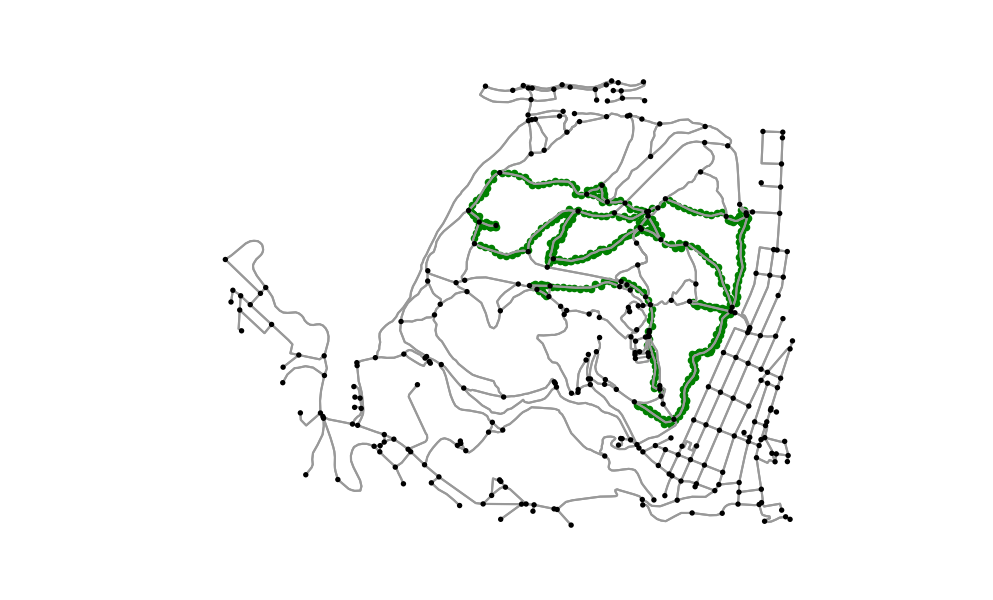
\includegraphics[width=0.9\textwidth]{./Imagenes/SimulatedTrack2Empty.png}
\caption{Muestra de simulación 2 (Experimentación sin datos).}
\label{figure:SimulatedTrack2}
\end{minipage}
\hfill 
\begin{minipage}{0.48\textwidth}
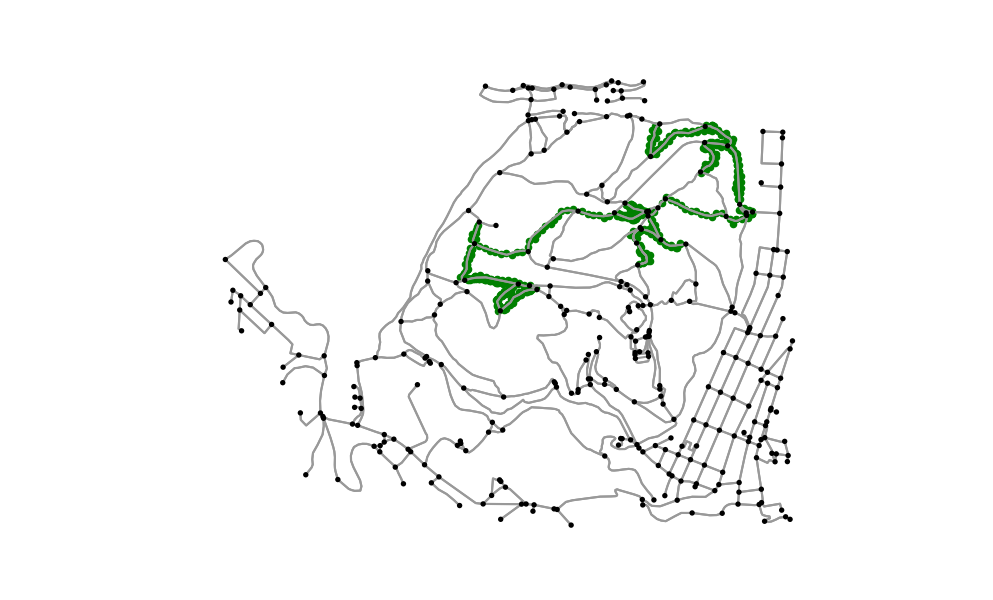
\includegraphics[width=0.9\textwidth]{./Imagenes/SimulatedTrack3Empty.png}
\caption{Muestra de simulación 3 (Experimentación sin datos).}
\label{figure:SimulatedTrack3}
\end{minipage}
\end{figure}
\newpage

Por una parte, en el mapa de calor resultante no se observan patrones observables, esto es debido a 
la elección pseudo-aleatoria de cada uno de los segmentos seleccionados.
\begin{figure}[!htb]
\begin{center}
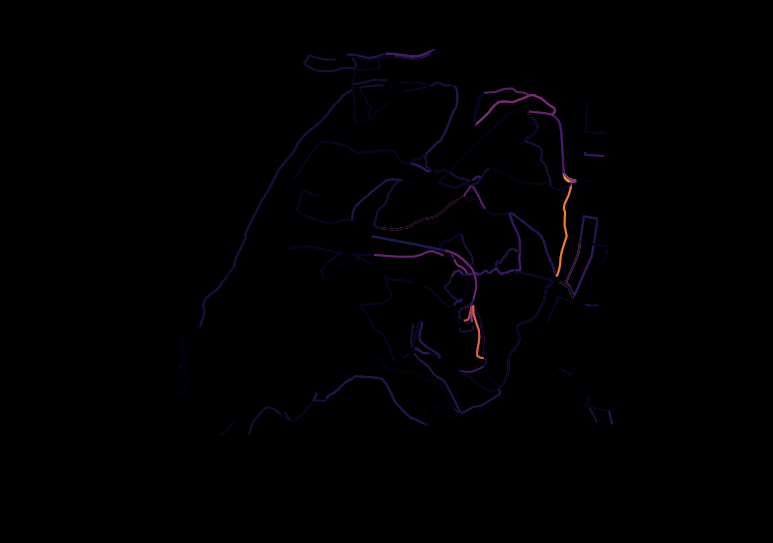
\includegraphics[width=0.7\textwidth]{./Imagenes/HeatMapEmpty.png}
\caption{Mapa de calor del conjunto de rutas simuladas en experimentación sin datos.}
\label{figure:SimulatedHeatMapEmpty}
\end{center}
\end{figure}
\newpage
Las distribuciones se observan constantes al valor parametrizado al que están asignados en caso 
de que no se encuentren datos para realizar la simulación (figura \ref{figure:SimulatedPointToPointEmpty}) por 
otra parte se observa la aletoriedad en forma de distribución normal de la distancia punto a proyección, que no 
corresponde a ningún comportamiento parametrizado (figura \ref{figure:SimulatedPointToProjectionEmpty}).
\begin{figure}[!htb]
\begin{minipage}{0.48\textwidth}
\centering
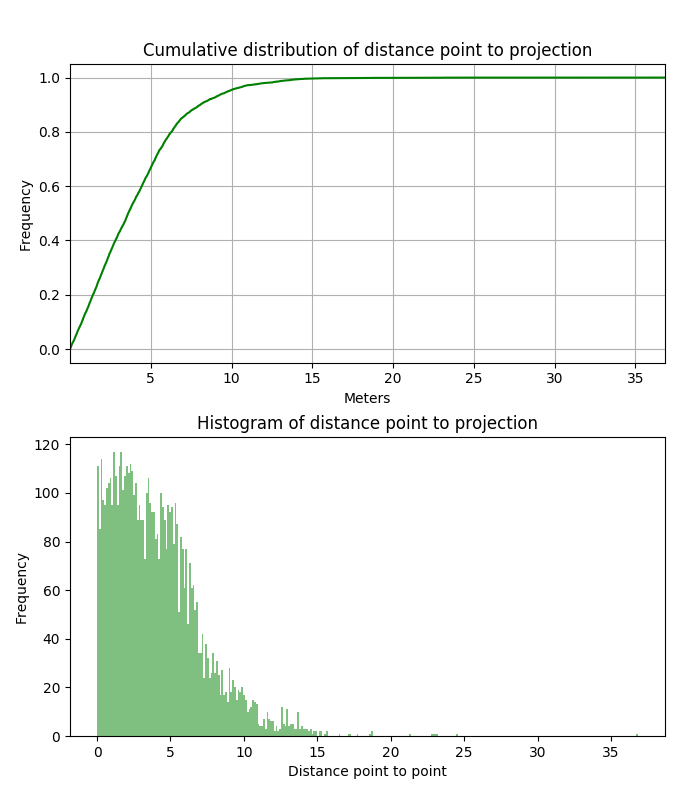
\includegraphics[width=0.9\textwidth]{./Imagenes/SimulateCumulativePointProjectionEmpty.png}
\caption{Muestra de análisis de simulación: Distancia punto a proyección en experimentación sin datos.}
\label{figure:SimulatedPointToProjectionEmpty}
\end{minipage}\hfill
\begin{minipage}{0.48\textwidth}
\centering
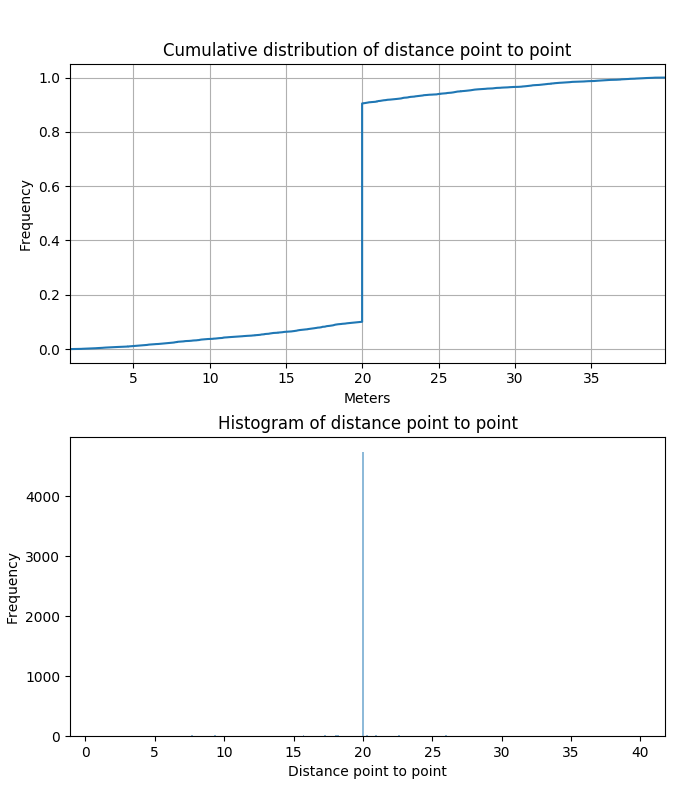
\includegraphics[width=0.9\textwidth]{./Imagenes/SimulateCumulativePointPointEmpty.png}
\caption{Muestra de análisis de simulación: Distancia punto a punto en experimentación sin datos.}
\label{figure:SimulatedPointToPointEmpty}
\end{minipage}
\end{figure}


\section{Experimentación con importación de datos reales}
Para la simulación, se ha alimentado al modelo con el análisis de las rutas reales de 10 km de distancia sobre 
el territorio del Castell de Bellver. Todas parten del origen de la entrada nordeste del recinto. Se han generado un total de 253 rutas. Posteriormente estas rutas han sido pasadas por el analizador con el objetivo de valorar si mantienen la misma distribución en las variables respecto el análisis de las rutas reales. Las figuras \ref{figure:SimulatedTrack1}.
\begin{figure}[!htb]
\centering
\begin{minipage}{0.70\textwidth}
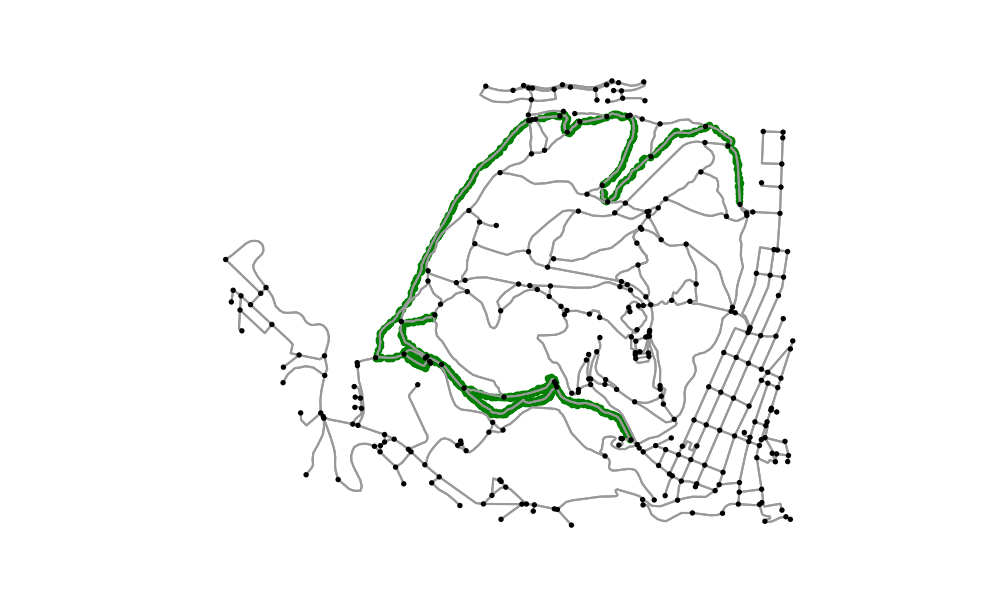
\includegraphics[width=0.9\textwidth]{./Imagenes/SimulatedTrack1.png}
\caption{Muestra de simulación 1 Experimentación con datos).}
\label{figure:SimulatedTrack1}
\end{minipage}
\begin{minipage}{0.48\textwidth}
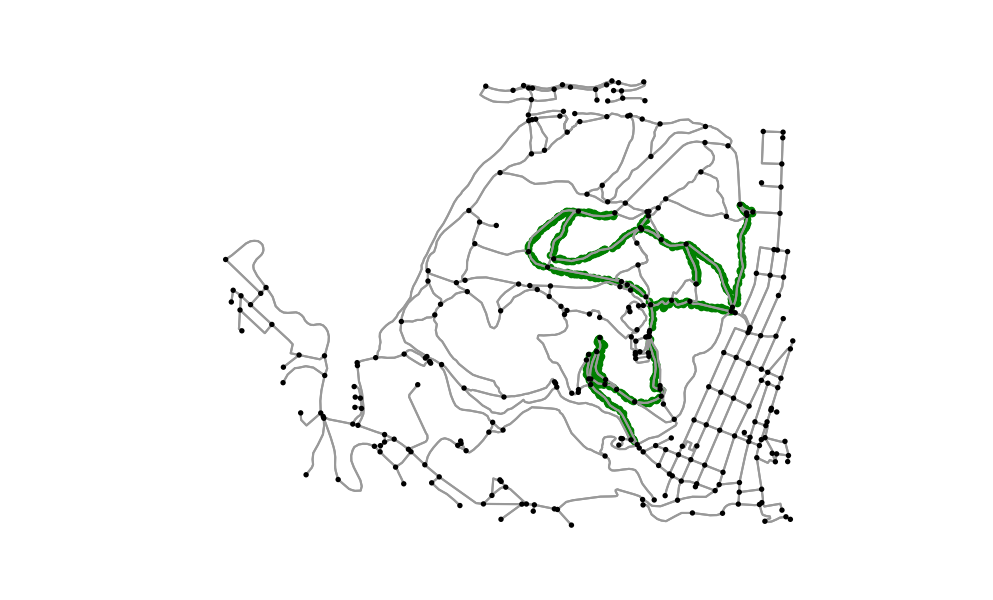
\includegraphics[width=0.9\textwidth]{./Imagenes/SimulatedTrack2.png}
\caption{Muestra de simulación 2 Experimentación con datos).}
\label{figure:SimulatedTrack2}
\end{minipage}
\hfill 
\begin{minipage}{0.48\textwidth}
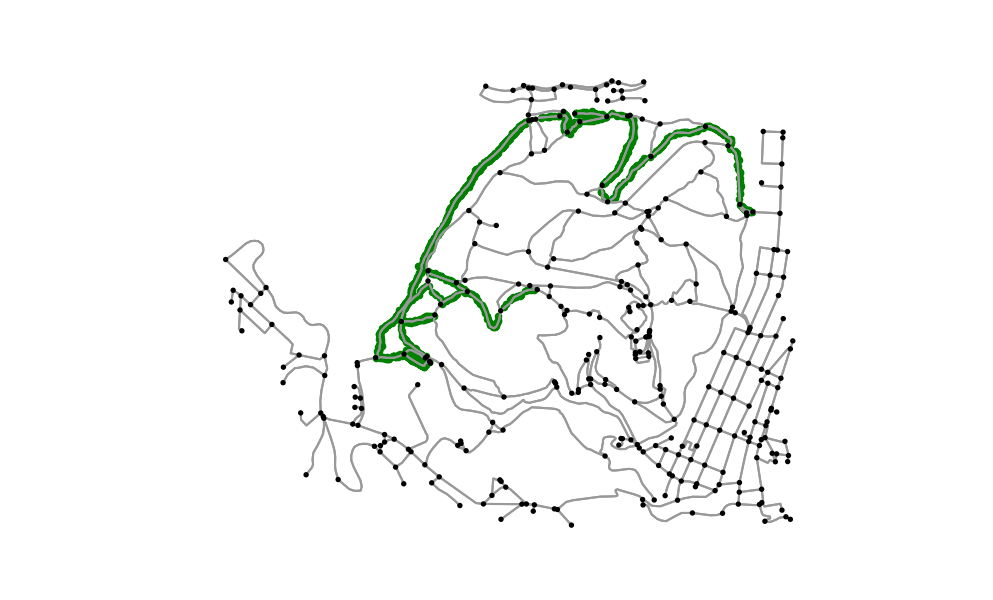
\includegraphics[width=0.9\textwidth]{./Imagenes/SimulatedTrack3.png}
\caption{Muestra de simulación 3 (Experimentación con datos).}
\label{figure:SimulatedTrack3}
\end{minipage}
\end{figure}
\newpage

La figura \ref{figure:SimulatedHeatMap} corresponde al mapa de calor del análisis de las generaciones. Se puede observar una trayectoria más definida, que se corresponde con el mapa de calor mostrado 
anteriormente en la figura \ref{figure:RealHeatMap}.
\begin{figure}[!htb]
\begin{center}
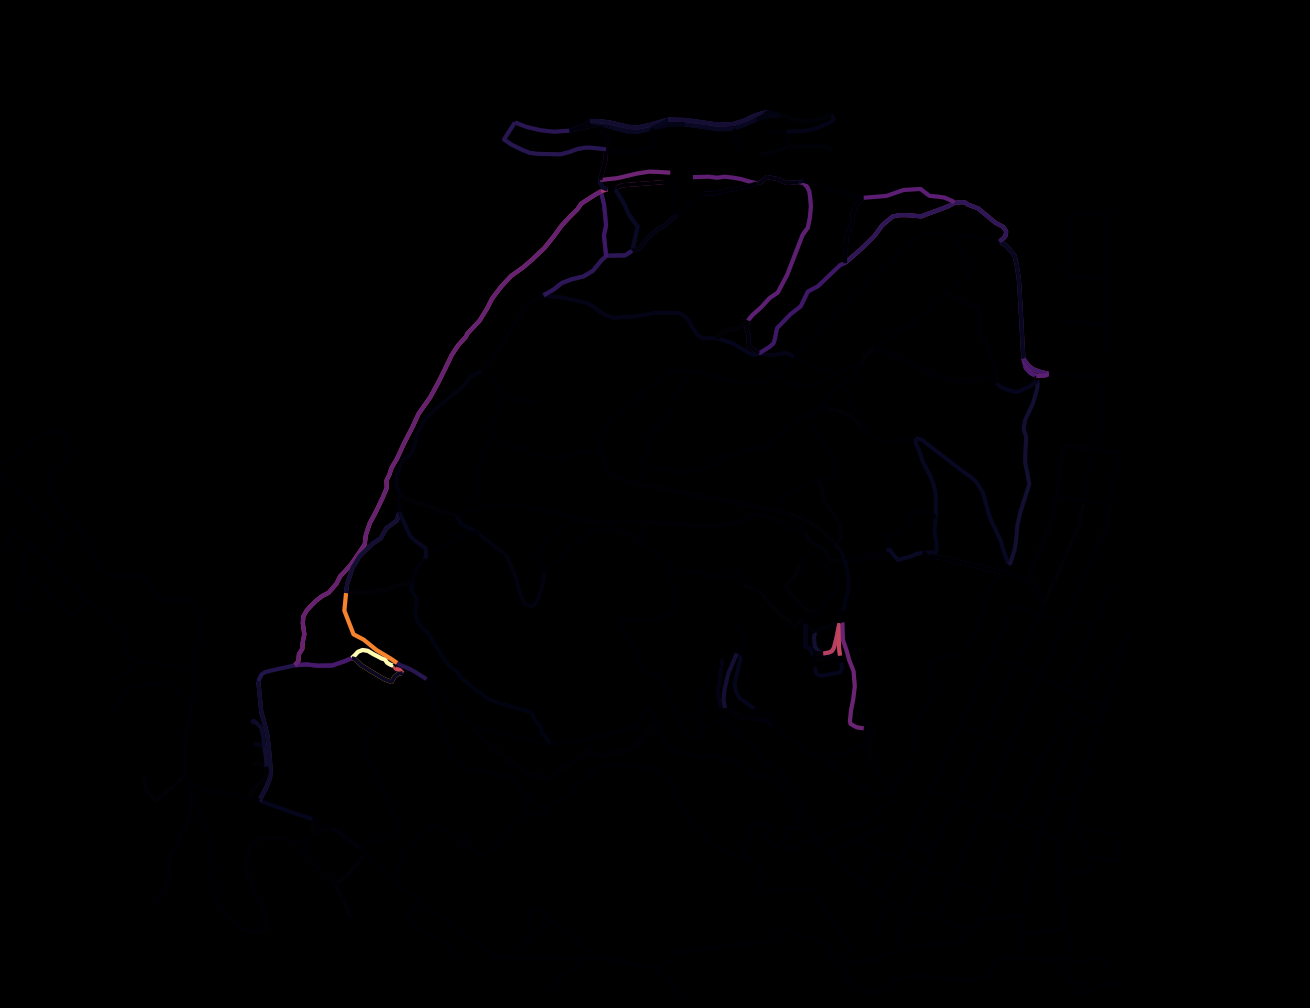
\includegraphics[width=0.7\textwidth]{./Imagenes/SimulatedHeatMap1.png}
\caption{Mapa de calor del conjunto de rutas simuladas en experimentación con datos.}
\label{figure:SimulatedHeatMap}
\end{center}
\end{figure}
Existen diversos aspectos que explican las diferencias entre los mapas de calor de las figuras \ref{figure:RealHeatMap} y \ref{figure:SimulatedHeatMap}. Las rutas simuladas tienen una distancia de 
10 kilometros, por lo que hacen inaccessibles ciertos caminos. Se aprecia que la parte norte y este del 
perímetro del bosque del Castell de Bellver es la zona más frecuente, que corresponde con las muestras 
reales. No obstante existen rutas que acceden a la parte sur del camino, con menos frecuencia, por lo 
que no son distingibles.
Las distribuciones corresponden. A nivel de distancia punto a punto se respeta completamente, en la 
distancia punto proyección encontramos una distribución normal mucho más acentuada.

\begin{figure}[!htb]
\begin{minipage}{0.48\textwidth}
\centering
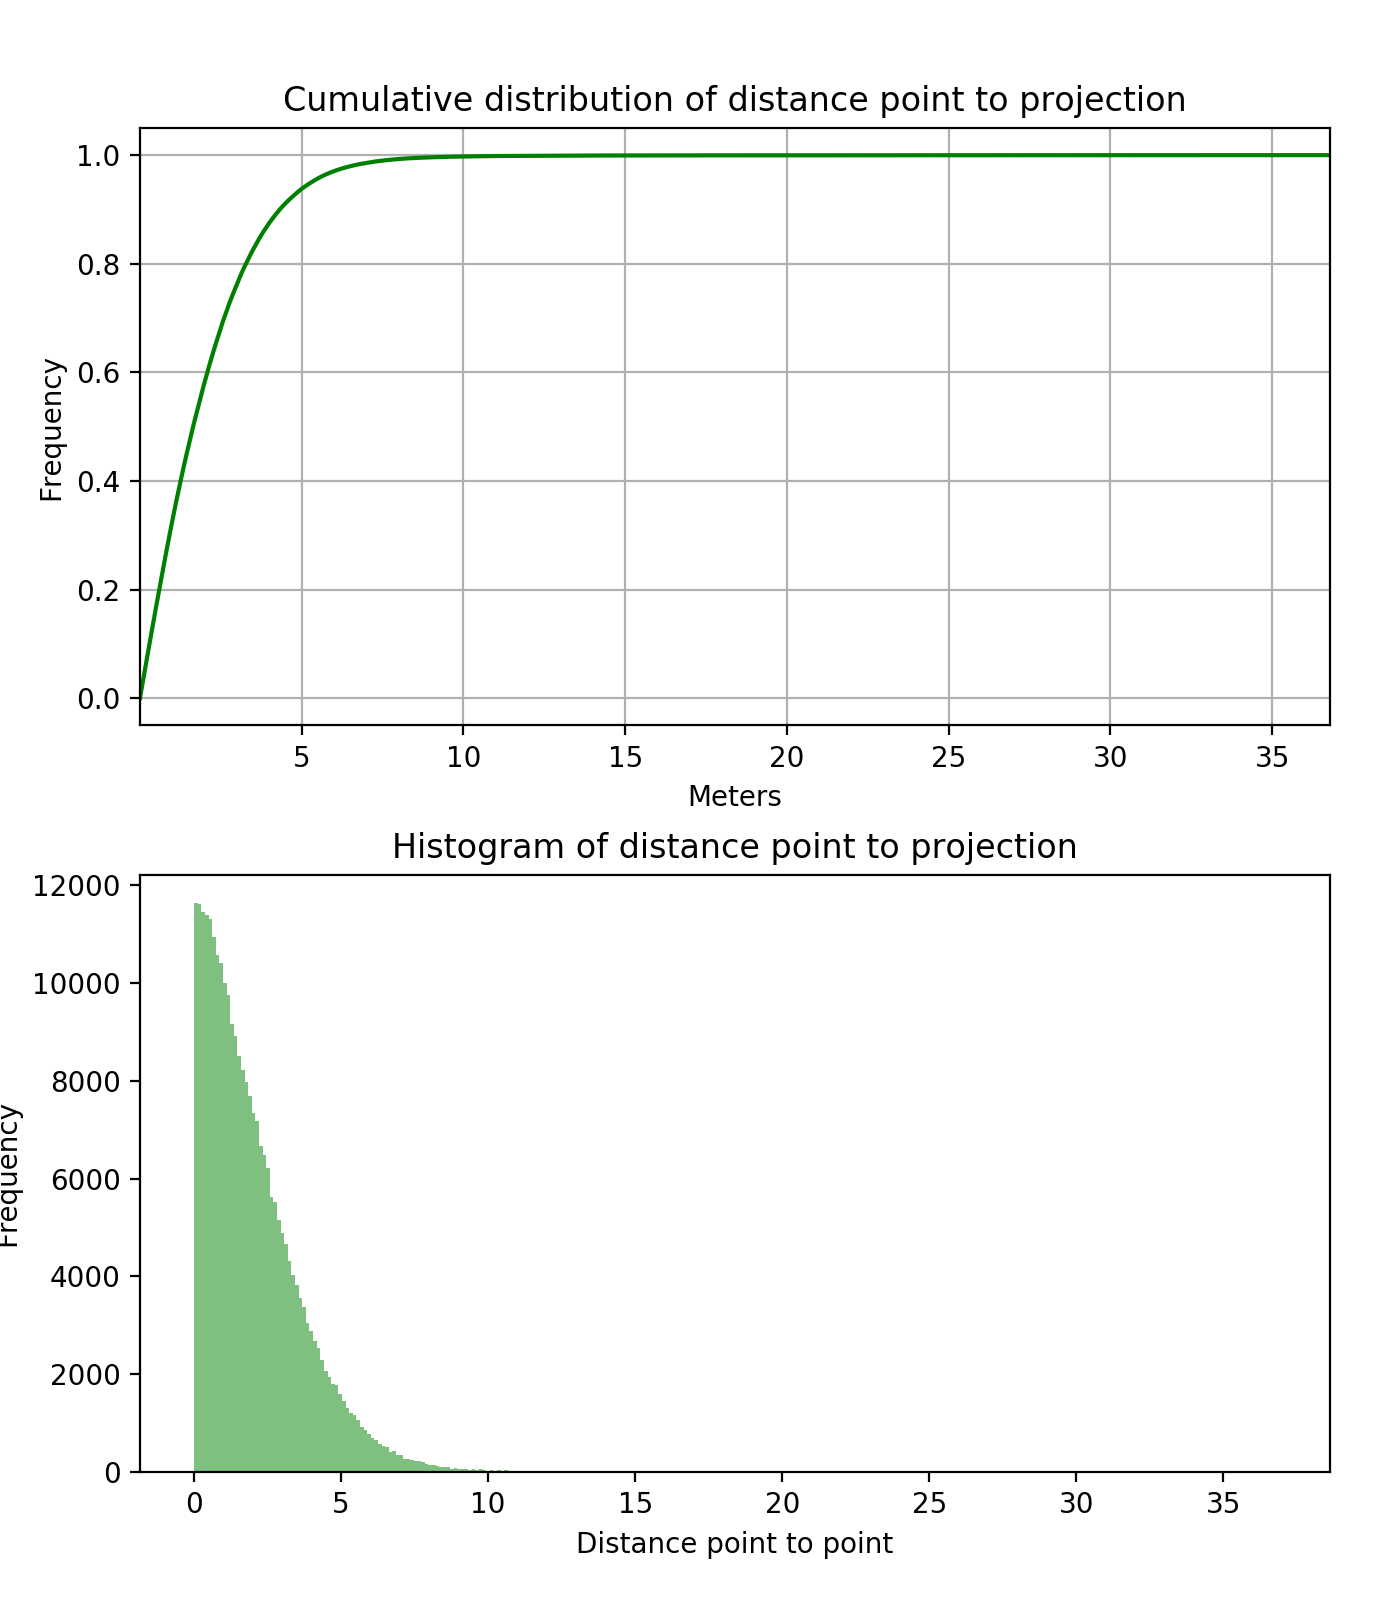
\includegraphics[width=0.9\textwidth]{./Imagenes/SimulateCumulativePointProjection.png}
\caption{Muestra de análisis de simulación: Distancia punto a proyección en experimentación con datos.}
\label{figure:SimulatedPointToProjection}
\end{minipage}\hfill
\begin{minipage}{0.48\textwidth}
\centering
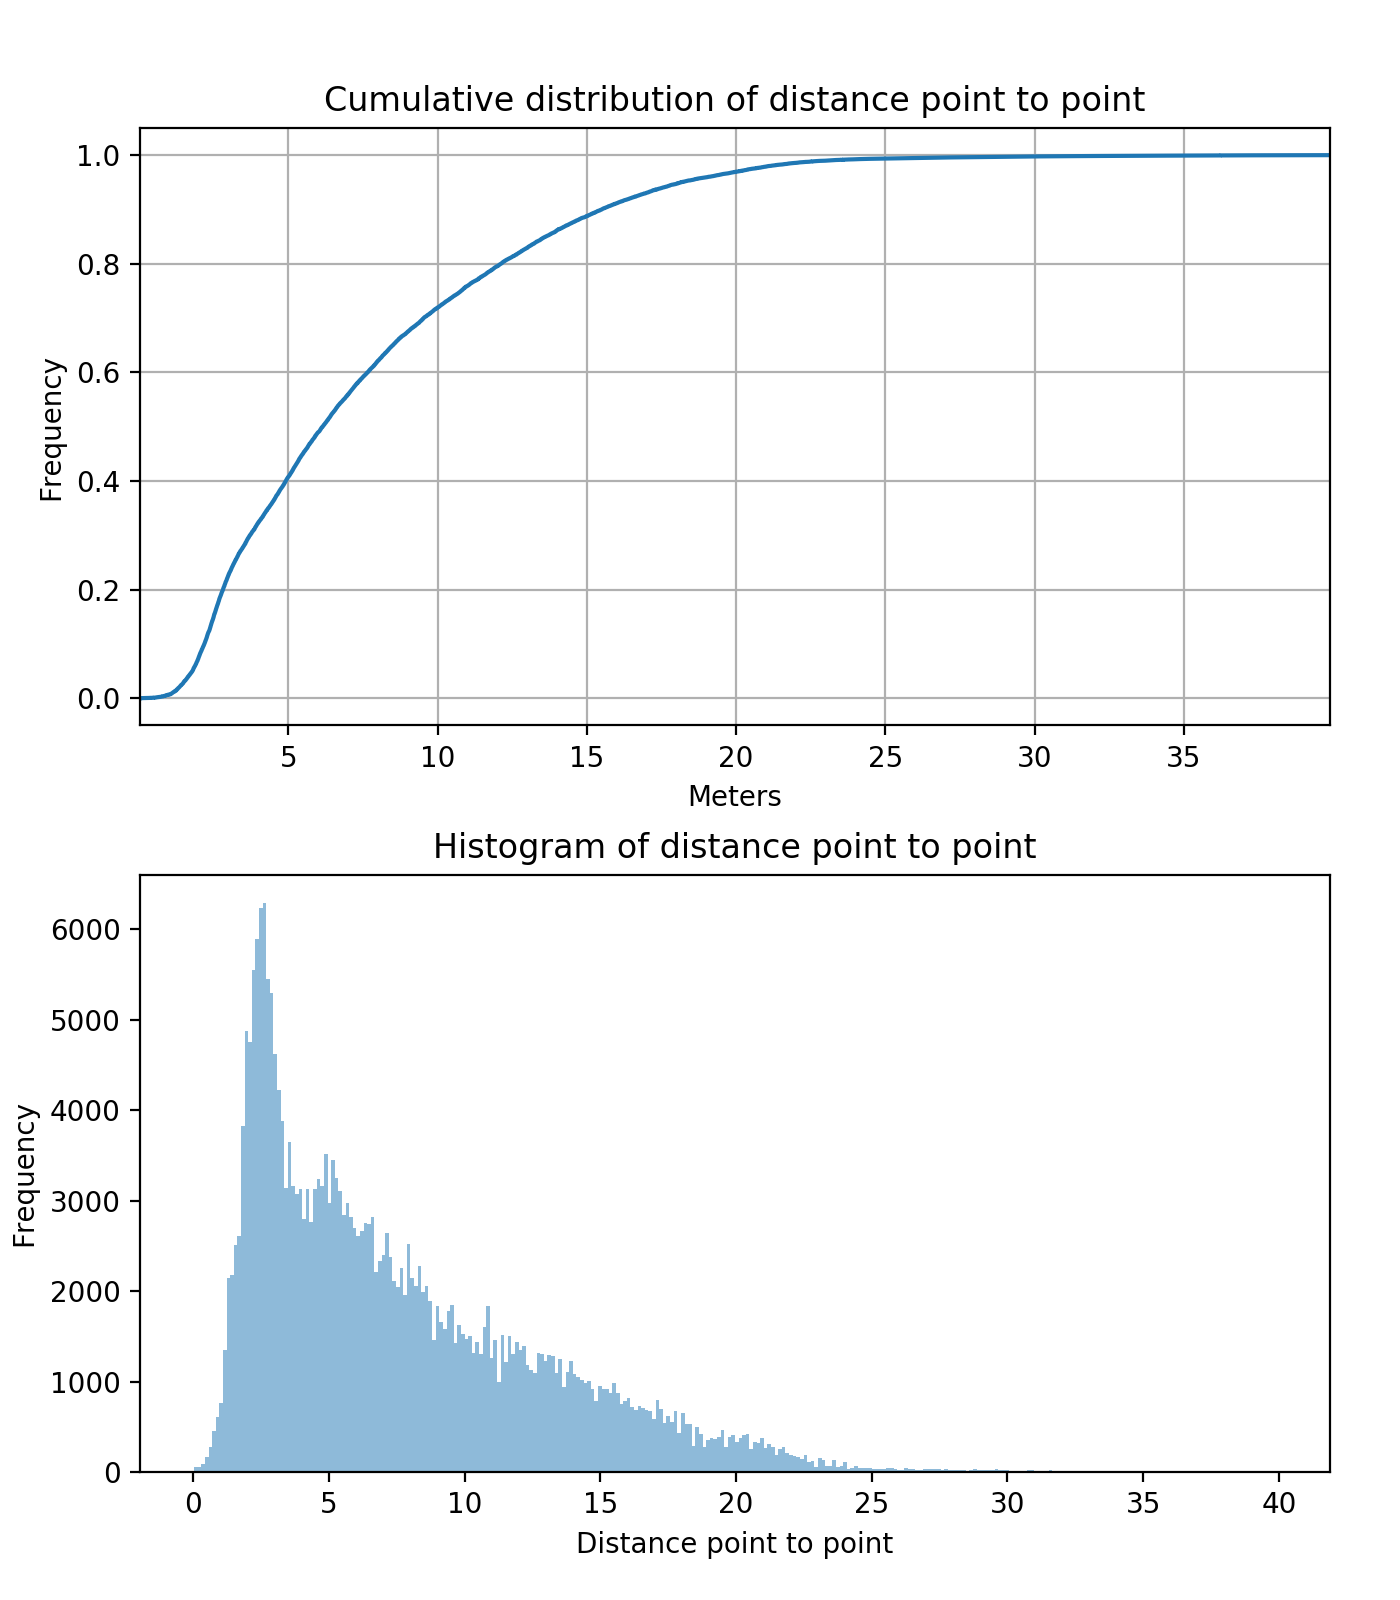
\includegraphics[width=0.9\textwidth]{./Imagenes/SimulateCumulativePointPoint.png}
\caption{Muestra de análisis de simulación: Distancia punto a punto en experimentación con datos.}
\label{figure:SimulatedPointToPoint}
\end{minipage}
\end{figure}

\subsection{Comparativa de resultados}
En las figuras \ref{figure:ComparativaReal} y \ref{figure:ComparativaEmpty} se observan los resultados de la distancia punto a punto entre y la comparativa con la distribución real. Se observa que con el uso de los datos 
procedentes del análisis se obtiene una distribución probabilística similar a la distribución real, mientras que 
sin estos datos, aparece una distribución única al valor parametrizado, en este caso 20 metros.

\begin{figure}[!htb]
\begin{minipage}{0.48\textwidth}
\centering
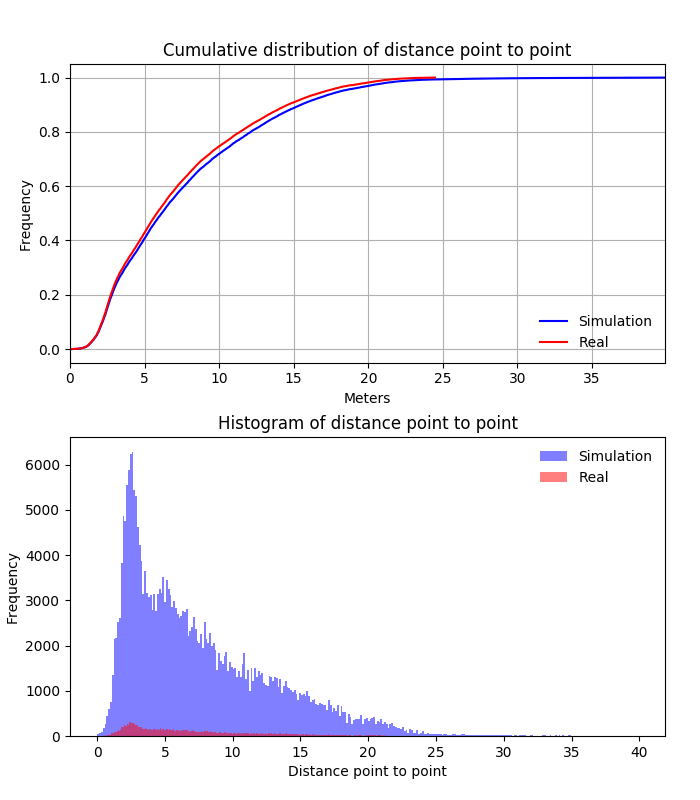
\includegraphics[width=0.9\textwidth]{./Imagenes/SimulationComparative.png}
\caption{Muestra de análisis de simulación: Distancia punto a proyección en experimentación con datos.}
\label{figure:ComparativaReal}
\end{minipage}\hfill
\begin{minipage}{0.48\textwidth}
\centering
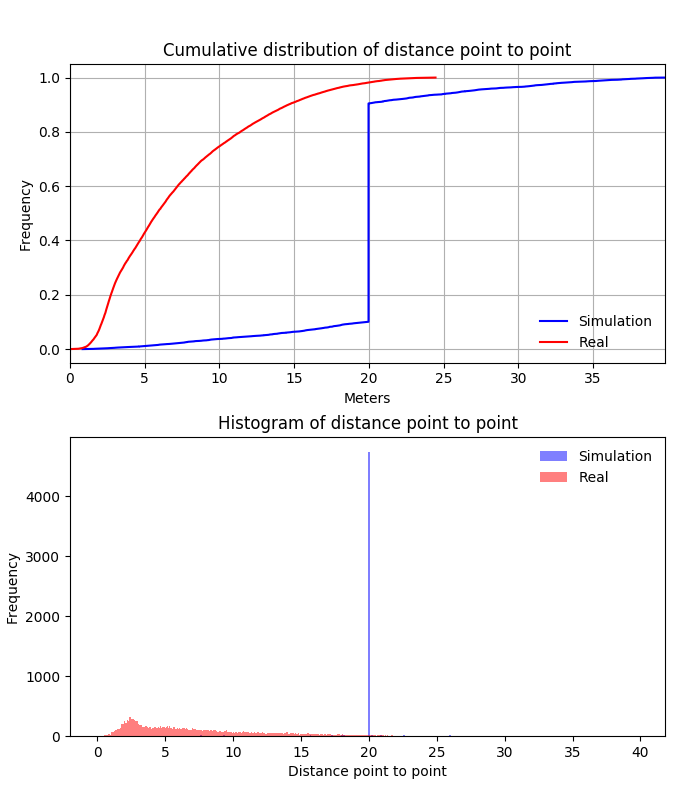
\includegraphics[width=0.9\textwidth]{./Imagenes/SimulationComparativeEmpty.png}
\caption{Muestra de análisis de simulación: Distancia punto a punto en experimentación con datos.}
\label{figure:ComparativaEmpty}
\end{minipage}
\end{figure}

Con esta información se aprecia que las simulaciones para este conjunto bajo de datos funciona con una alta similitud a las rutas reales proporcionadas.